\subsection{\lr{Overall Results}}
\begin{figure}[H]
    \centering
    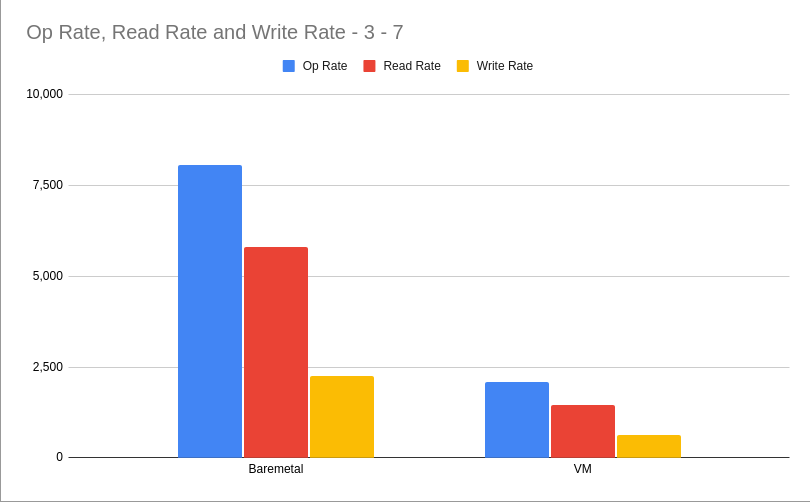
\includegraphics[scale=0.5]{pictures/cassandra/overall_result-3-7.png}
    \caption{ مقایسه تعداد عملیات‌ها در ثانیه در تست \lr{3-7}}
    \label{fig:cassandra:init:overall_results1}
\end{figure}
\begin{figure}[H]
    \centering
    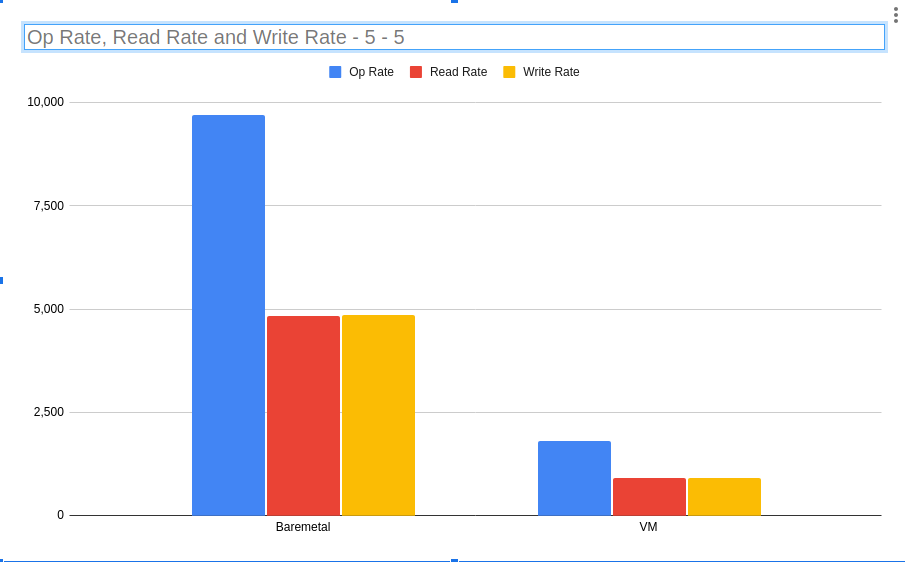
\includegraphics[scale=0.45]{pictures/cassandra/overall_result-5-5.png}
    \caption{ مقایسه تعداد عملیات‌ها در ثانیه در تست \lr{5-5}}
    \label{fig:cassandra:init:overall_results1}
\end{figure}
\begin{figure}[H]
    \centering
    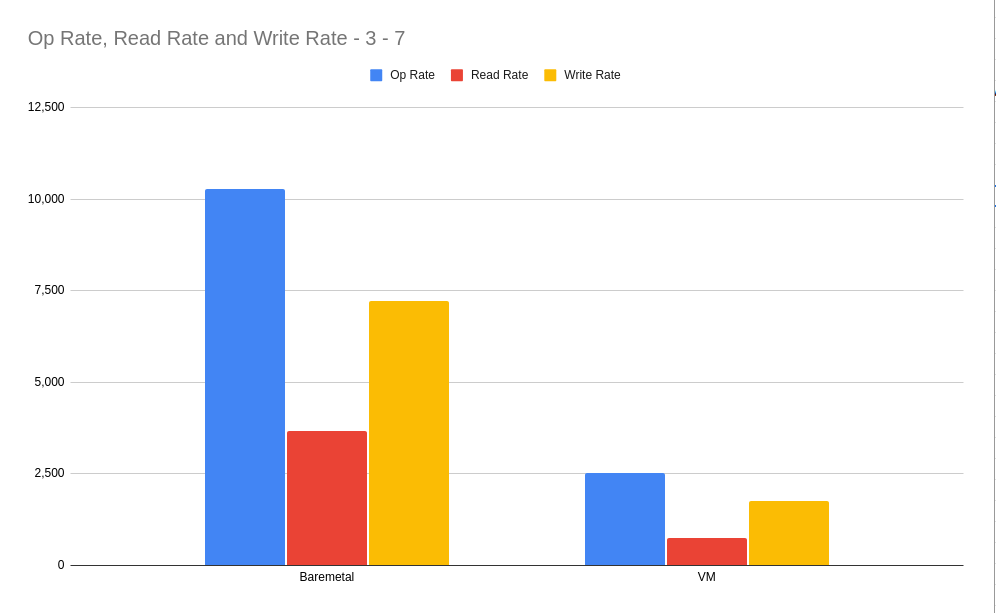
\includegraphics[scale=0.5]{pictures/cassandra/overall_result-7-3.png}
    \caption{ مقایسه تعداد عملیات‌ها در ثانیه در تست \lr{7-3}}
    \label{fig:cassandra:init:overall_results1}
\end{figure}
همانطور که در شکل‌های بالا می‌توان متوجه شد همانند تست‌های redis 
، احتمالا به دلیل وجود منابع بیشتر و نیز عملیات نسبتا سرراست‌تر در ماشین حقیقی،‌ به صورت کلی در این سیستم عملکرد کلی سیستم حقیقی تقریبا ۴ برابر بهتر از ماشین مجازی است.